% !TEX encoding = UTF-8
% !TEX program = pdflatex
% !TEX spellcheck = it_IT
% !BIB TS-program = biber

\documentclass[a4paper,12pt]{thesis}
\usepackage[T1]{fontenc}
\usepackage[utf8]{inputenc}
\usepackage[italian]{babel}
\usepackage{csquotes}
\usepackage{newcent}
\usepackage{graphicx}
\usepackage{listings}
%\usepackage{xcolor}
\usepackage[table,svgnames]{xcolor}
\usepackage{textcomp}
\usepackage{booktabs}
\usepackage{longtable}
\usepackage{array}
\usepackage{url,amsfonts,epsfig}
\usepackage{lmodern}
\usepackage{vmargin}
\usepackage{amsmath}
\usepackage{indentfirst}
\usepackage{graphicx}
\usepackage{color}
\usepackage{setspace}
\usepackage{siunitx}
\usepackage{footnote}
\usepackage{pgfplots}
\usepackage{ctable}
\usepackage{afterpage}
\usepackage{latexsym}
\usepackage{standalone}
\usepackage{graphicx}
\usepackage[style=numeric-comp,useprefix,hyperref,backend=biber]{biblatex}
\usepackage{float}
\usepackage{rotating}
\usepackage{makecell}
\usepackage{multirow}
\usepackage{pifont}
\usepackage{tabstackengine}
\pgfplotsset{width=10cm,height=14cm,compat=1.18}
\newcommand{\xmark}{\ding{55}}
\DeclareSortingTemplate{nonenyt}{
  \sort{\citeorder}
  \sort{
    \field{presort}
  }
  \sort[final]{
    \field{sortkey}
  }
  \sort{
    \field{sortname}
    \field{author}
    \field{editor}
    \field{translator}
    \field{sorttitle}
    \field{title}
  }
  \sort{
    \field{sortyear}
    \field{year}
  }
  \sort{
    \field{sorttitle}
    \field{title}
  }
  \sort{
    \field{volume}
    \literal{0}
  }
}
\ExecuteBibliographyOptions{sorting=nonenyt}
%\addbibresource{bibliografia.bib}
% \addbibresource{bibliografia_nuova.bib} % bibliografia del template precedente
\addbibresource{bibliografia_visioncaption.bib}

\newcommand{\Csh}{C{\lserif\#}}

\usepackage{caption, subcaption}
\captionsetup[sub]{labelformat=simple}
\renewcommand{\thesubfigure}{(\alph{subfigure})}
\usepackage{calligra}
\usepackage[T1]{fontenc}
\usepackage{inconsolata}
\definecolor{bluekeywords}{rgb}{0.13,0.13,1}
\definecolor{greencomments}{rgb}{0,0.5,0}
\definecolor{redstrings}{rgb}{0.9,0,0}
\definecolor{dkgreen}{rgb}{0,0.6,0}
\definecolor{gray}{rgb}{0.5,0.5,0.5}
\definecolor{darkblue}{rgb}{0.0,0.0,0.6}
\definecolor{lightblue}{rgb}{0.0,0.0,0.9}
\definecolor{cyan}{rgb}{0.0,0.6,0.6}
\definecolor{darkred}{rgb}{0.6,0.0,0.0}
\definecolor{mauve}{rgb}{0.58,0,0.82}

\lstset{
language=[Sharp]C,
showspaces=false,
showtabs=false,
breaklines=true,
showstringspaces=false,
breakatwhitespace=true,
escapeinside={(*@}{@*)},
commentstyle=\color{greencomments},
keywordstyle=\color{bluekeywords}\bfseries,
stringstyle=\color{redstrings},
basicstyle=\ttfamily
}

\lstset{
  basicstyle=\ttfamily\footnotesize,
  columns=fullflexible,
  showstringspaces=false,
  numbers=left,                   % where to put the line-numbers
  numberstyle=\tiny\color{gray},  % the style that is used for the line-numbers
  stepnumber=1,
  numbersep=5pt,                  % how far the line-numbers are from the code
  backgroundcolor=\color{white},      % choose the background color. You must add \usepackage{color}
  showspaces=false,               % show spaces adding particular underscores
  showstringspaces=false,         % underline spaces within strings
  showtabs=false,                 % show tabs within strings adding particular underscores
  frame=none,                   % adds a frame around the code
  rulecolor=\color{black},        % if not set, the frame-color may be changed on line-breaks within not-black text (e.g. commens (green here))
  tabsize=2,                      % sets default tabsize to 2 spaces
  captionpos=b,                   % sets the caption-position to bottom
  breaklines=false,                % sets automatic line breaking
  breakatwhitespace=false,        % sets if automatic breaks should only happen at whitespace
  title=\lstname,                   % show the filename of files included with \lstinputlisting;
                                  % also try caption instead of title
  commentstyle=\color{gray}\upshape
}

\lstdefinelanguage{XML}
{
  morestring=[s][\color{mauve}]{"}{"},
  morestring=[s][\color{black}]{>}{<},
  morecomment=[s]{<?}{?>},
  morecomment=[s][\color{dkgreen}]{<!--}{-->},
  stringstyle=\color{black},
  identifierstyle=\color{lightblue},
  keywordstyle=\color{lightblue},
  morekeywords={xmlns,xsi,noNamespaceSchemaLocation,type,id,x,y,source,target,version,tool,transRef,roleRef,objective,eventually}% list your attributes here
}

\lstdefinelanguage{json}{
    basicstyle=\normalfont\ttfamily,
    numbers=left,
    numberstyle=\scriptsize,
    stepnumber=1,
    numbersep=8pt,
    showstringspaces=false,
    breaklines=true,
    frame=lines,
    backgroundcolor=\color{background},
    literate=
     *{0}{{{\color{numb}0}}}{1}
      {1}{{{\color{numb}1}}}{1}
      {2}{{{\color{numb}2}}}{1}
      {3}{{{\color{numb}3}}}{1}
      {4}{{{\color{numb}4}}}{1}
      {5}{{{\color{numb}5}}}{1}
      {6}{{{\color{numb}6}}}{1}
      {7}{{{\color{numb}7}}}{1}
      {8}{{{\color{numb}8}}}{1}
      {9}{{{\color{numb}9}}}{1}
      {:}{{{\color{punct}{:}}}}{1}
      {,}{{{\color{punct}{,}}}}{1}
      {\{}{{{\color{delim}{\{}}}}{1}
      {\}}{{{\color{delim}{\}}}}}{1}
      {[}{{{\color{delim}{[}}}}{1}
      {]}{{{\color{delim}{]}}}}{1},
}


\graphicspath{{images/}}
\usepackage[hyperindex]{hyperref} %per l'indice interattivo
\hypersetup{colorlinks=true, linkcolor=black, citecolor=black} %per
\setmarginsrb{35mm}{30mm}{30mm}{30mm}{0mm}{10mm}{0mm}{10mm}

\title{Sviluppo di un ambiente virtuale con digital twins per la videosorveglianza}
\author{Renato Esposito}
\date{\today}

\begin{document}
\hypersetup{pageanchor=false}
%%%% Opzione per interlinea 2
\baselineskip 1.6em

%% FRONTESPIZIO
{ \thispagestyle{empty}

\vskip 1cm \large \centerline{\textsc{Università degli Studi di Napoli "Parthenope"}}

\centerline {\textsc{Dipartimento di Scienze e Tecnologie}}

\centerline {\small\textsc{Corso di laurea in Informatica}}

\vskip 1.0cm

\begin{center}

\includegraphics[scale=0.7]{Immagini/logouni.png}
%
\includegraphics[scale=0.45]{Immagini/logouni.png}
\end{center}

\vskip 0.5cm

\large \centerline {\textsc{Elaborato finale di Laurea}}

\vskip 1.0cm
\Large \center {VISIONE ASSISTIVA: DESCRIZIONE AMBIENTALE VOCALE IN TEMPO REALE PER IPOVEDENTI CON VISION-LANGUAGE MODEL}
\vskip 1.0cm
%\small \center{sottotitolo}
%\vskip 1cm

\large
\begin{minipage}[t]{7cm}
\textsc{Relatore}

\textbf{Prof.ssa Paola Barra}
\vskip 1cm
%\textsc{Correlatore}
%\textbf{Dott. Antonio Pigna}

\end{minipage}
\hfill
\begin{minipage}[t]{5cm}
\textsc{Candidato}

\textbf{Samuel Arenella }
\textbf{\\Matricola Matr. \\0124002529}

\end{minipage}
\vskip 3cm
\Large \centerline {Anno Accademico 2025/2026}
\vfill \eject}
\pagenumbering{Roman}
% Commenta dalla riga successiva per generare il frontespizio
\newpage
\newpage
\markboth{Index}{Index}
\tableofcontents
% \listoffigures
% \listoftables
\clearpage
\pagenumbering{arabic}
\hypersetup{pageanchor=true}

\chapter{Introduzione}
\label{cap:introduzione}

\section{Contesto e motivazione}

La vista consente di acquisire rapidamente una grande quantità di informazioni
sull'ambiente circostante: permette di riconoscere oggetti e persone,
interpretare segnali ed etichette, leggere testi e comprendere la disposizione
degli elementi nello spazio. Quando questa capacità è ridotta o assente,
l'accesso a tali informazioni può richiedere strumenti assistivi oppure il
supporto di altre persone.

La disabilità visiva comprende condizioni differenti e non corrisponde a
un'unica esperienza percettiva. Può interessare la visione da vicino o da
lontano e presentarsi con livelli diversi di gravità. Alcune persone conservano
una capacità visiva parziale, mentre altre non possono utilizzare la vista per
accedere alle informazioni presenti nell'ambiente. Con il termine
\emph{ipovisione} si indica, in questo lavoro, una condizione nella quale è
presente un residuo visivo, ma la percezione disponibile può non essere
sufficiente per riconoscere con affidabilità dettagli, testi o oggetti in ogni
condizione. Anche fattori come illuminazione, contrasto e organizzazione dello
spazio possono influire sull'autonomia nelle attività quotidiane. Secondo
l'Organizzazione Mondiale della Sanità, almeno 2,2 miliardi di persone nel
mondo presentano una compromissione della visione da vicino o da lontano
\cite{who_blindness_vision_impairment_2026}.

In questo contesto, le tecnologie assistive possono contribuire a rendere
accessibili attraverso il canale uditivo informazioni originariamente
disponibili soltanto in forma visiva. I progressi nella computer vision, nei
modelli visivo-linguistici e nella sintesi vocale rendono oggi possibile
analizzare un'immagine, produrne una descrizione testuale e convertirla in
parlato. Affinché questo processo sia realmente utile, tuttavia, non è
sufficiente generare una descrizione: occorre stabilire quando fornirla, quale
elemento descrivere e come evitare informazioni ripetitive o poco pertinenti.

% Qui puoi aggiungere, se lo desideri, una breve motivazione personale
% che spieghi perché hai scelto questo specifico problema di tesi.

\section{Problema di ricerca}

L'ambiente quotidiano è dinamico e contiene una quantità elevata di
informazioni visive. Una descrizione continua e indiscriminata rischierebbe di
sovraccaricare l'utente, sovrapporre più messaggi vocali e ripetere contenuti
già comunicati. Al contrario, un sistema attivabile soltanto mediante comandi
espliciti richiederebbe all'utente di formulare ogni volta una richiesta,
anche quando avrebbe bisogno semplicemente di conoscere un cambiamento
avvenuto nelle vicinanze.

Si presenta quindi la necessità di conciliare due esigenze complementari:
mantenere una consapevolezza generale di ciò che accade nell'ambiente e
consentire all'utente di richiedere informazioni mirate su un elemento
specifico. Il sistema deve inoltre limitare la latenza, evitare descrizioni
ridondanti e comunicare soltanto informazioni che possano essere formulate con
un livello adeguato di affidabilità.

La domanda che guida il presente lavoro può essere formulata nel modo
seguente:

\begin{quote}
\emph{È possibile realizzare un sistema browser-based che fornisca
descrizioni vocali contestuali, sia automaticamente sia attraverso un gesto di
puntamento, senza richiedere hardware proprietario?}
\end{quote}

\section{Obiettivi del progetto}

L'obiettivo della tesi è la progettazione e lo sviluppo di VisionCaption, un
sistema di visione assistita rivolto a persone cieche e ipovedenti, capace di
generare descrizioni vocali della scena osservata dalla fotocamera di un
dispositivo. L'applicazione è concepita per funzionare tramite browser, così da
poter essere utilizzata su dispositivi comuni, come computer, smartphone e
tablet, senza dipendere da uno specifico visore o da sensori proprietari.

Le descrizioni devono essere brevi, comprensibili e formulate in lingua
italiana. L'obiettivo non è sostituire gli ausili tradizionali per
l'orientamento e la mobilità, né realizzare un dispositivo medico, ma fornire
un ulteriore canale di accesso alle informazioni visive. Il sistema è quindi
pensato come supporto alla comprensione del contesto e non come fonte unica
sulla quale basare decisioni relative alla sicurezza personale.

Per rispondere a esigenze differenti, VisionCaption prevede due modalità di
interazione: una modalità automatica, orientata alla consapevolezza generale
dell'ambiente, e una modalità di puntamento, destinata all'esplorazione
intenzionale di un oggetto.

\section{Modalità di interazione}

\subsection{Modalità automatica}

La modalità automatica non richiede un intervento esplicito da parte
dell'utente. Il sistema osserva il flusso proveniente dalla fotocamera e produce
una nuova descrizione quando rileva un cambiamento sufficientemente rilevante
nella scena. In questo modo l'utente può ricevere informazioni su ciò che lo
circonda durante le normali attività quotidiane, evitando che una scena
sostanzialmente invariata generi continuamente la stessa caption.

Questa modalità privilegia quindi la continuità dell'assistenza, ma deve
mantenere un equilibrio tra tempestività e quantità delle informazioni. Una
frequenza eccessiva renderebbe infatti l'audio invasivo, mentre una frequenza
troppo bassa potrebbe omettere cambiamenti utili.

\subsection{Modalità di puntamento}

La modalità di puntamento offre un'interazione più intenzionale. L'utente può
indicare con il dito l'elemento sul quale desidera ricevere informazioni,
senza dover formulare verbalmente una domanda o selezionare manualmente una
regione dello schermo. Il sistema riconosce una posa di puntamento mantenuta in
modo stabile, interpreta la direzione indicata e genera una descrizione
specifica del possibile referente.

Questa modalità può essere impiegata, ad esempio, per conoscere la natura di
un oggetto, distinguerlo dagli elementi vicini oppure leggere il testo visibile
su un'etichetta o una confezione. Il gesto deittico costituisce così un
collegamento diretto tra l'intenzione dell'utente e la porzione di ambiente da
descrivere.

\section{Contributo del lavoro}

Il contributo del progetto non consiste nella definizione di un nuovo modello
fondazionale di intelligenza artificiale, ma nell'integrazione di tecniche di
visione artificiale, modelli multimodali e sintesi vocale all'interno di
un'unica esperienza assistiva. L'aspetto centrale è la coesistenza di due
strategie complementari: una descrizione automatica sensibile ai cambiamenti
della scena e una descrizione attivata da un gesto naturale di puntamento.

La scelta di un'interfaccia browser-based mira inoltre a ridurre la dipendenza
da piattaforme e dispositivi specifici. Il lavoro affronta pertanto non solo il
riconoscimento del contenuto visivo, ma anche problemi legati alla selezione
dell'informazione, alla latenza, alla ripetizione delle caption e alla
semplicità dell'interazione.

\section{Organizzazione della tesi}

Il presente capitolo introduce il contesto, il problema e gli obiettivi del
lavoro. Il Capitolo~\ref{cap:tecnologie} presenta le principali tecnologie
utilizzate, mentre il capitolo dedicato allo stato dell'arte confronta
VisionCaption con le soluzioni assistive esistenti. I capitoli successivi
descrivono la progettazione del sistema, le scelte implementative e la
valutazione dei risultati ottenuti.

% Aggiorna l'ultimo periodo quando l'indice definitivo dei capitoli sarà
% stabilito, indicando esplicitamente il contenuto di ciascun capitolo.

\chapter{Tecnologie utilizzate}
\label{cap:tecnologie}

VisionCaption combina tecnologie web, computer vision e intelligenza
artificiale. In questo capitolo vengono presentate la natura e le
caratteristiche principali delle tecnologie adottate. Il modo in cui esse sono
integrate nell'architettura e nelle due modalità operative viene invece
affrontato nei capitoli di approfondimento e di sviluppo del sistema.

\section{Linguaggio e gestione del progetto}

\subsection{Python}
Python è un linguaggio di programmazione ad alto livello, multipiattaforma e di
uso generale. Utilizza una tipizzazione dinamica e dispone di costrutti per la
programmazione procedurale, a oggetti e funzionale. Il suo ecosistema comprende
numerose librerie per lo sviluppo web, il calcolo numerico, la computer vision
e il machine learning.

Python supporta inoltre la programmazione asincrona attraverso il modello
\texttt{async}/\texttt{await}, che consente di coordinare operazioni di
ingresso e uscita senza associare necessariamente un thread a ciascuna
operazione.

\subsection{uv}
\textit{uv} è uno strumento per la gestione di progetti e pacchetti Python.
Permette di creare ambienti virtuali, risolvere e installare le dipendenze e
generare un file di lock. Quest'ultimo registra le versioni esatte dei
pacchetti, rendendo riproducibile l'ambiente di esecuzione.

\subsection{Hatchling}
Hatchling è un backend di build conforme allo standard PEP 517. Il suo compito
è trasformare il codice sorgente e i metadati di un progetto Python in
distribuzioni installabili, come wheel e source distribution.

\section{Tecnologie web e comunicazione}

\subsection{Browser web}
Il browser è l'ambiente software che interpreta ed esegue le applicazioni web.
Oltre a HTML, CSS e JavaScript, espone API standard per accedere alle
funzionalità del dispositivo, tra cui fotocamera, riproduzione audio,
connessioni di rete e disegno bidimensionale. L'impiego di standard web
permette di realizzare applicazioni multipiattaforma senza richiedere hardware
proprietario.

\subsection{FastAPI}
FastAPI è un framework web open source per la realizzazione di API in Python.
È basato sulle annotazioni di tipo del linguaggio e utilizza Starlette per le
funzionalità web e Pydantic per la gestione dei dati. Supporta applicazioni
asincrone, API HTTP, WebSocket e generazione automatica della documentazione
OpenAPI.

\subsection{Uvicorn e ASGI}
Uvicorn è un server web per applicazioni Python conformi allo standard ASGI
(\textit{Asynchronous Server Gateway Interface}). ASGI definisce l'interfaccia
tra server e applicazione e, a differenza del precedente standard sincrono
WSGI, supporta connessioni di lunga durata e comunicazioni asincrone come i
WebSocket.

\subsection{WebSocket}
WebSocket è un protocollo di comunicazione che stabilisce un canale persistente
e bidirezionale tra client e server. Dopo una fase iniziale di handshake, le
due parti possono inviare messaggi in modo indipendente sulla stessa
connessione. Il protocollo è indicato con \texttt{WS}; la variante
\texttt{WSS} aggiunge la protezione crittografica fornita da TLS.

\subsection{JSON}
JSON (\textit{JavaScript Object Notation}) è un formato testuale per lo scambio
di dati strutturati. Rappresenta le informazioni mediante oggetti, array,
stringhe, numeri, valori booleani e valori nulli. È indipendente dal linguaggio
di programmazione ed è ampiamente utilizzato nelle API web.

\subsection{Base64}
Base64 è una codifica che rappresenta dati binari attraverso un insieme di
caratteri ASCII. Consente quindi di inserire immagini, audio o altri contenuti
binari in formati testuali come JSON. Non comprime né cifra le informazioni e
produce una rappresentazione più grande rispetto ai dati originali.

\subsection{HTTPX}
HTTPX è un client HTTP per Python dotato di interfacce sincrone e asincrone.
Supporta funzionalità quali connessioni persistenti, timeout, streaming delle
risposte e protocolli HTTP/1.1 e HTTP/2. È pensato per effettuare richieste di
rete senza rinunciare al modello asincrono del linguaggio.

\section{Validazione e osservabilità}

\subsection{Pydantic}
Pydantic è una libreria per la validazione, la serializzazione e il parsing dei
dati basata sulle annotazioni di tipo di Python. Attraverso modelli dichiarativi
consente di verificare la struttura dei valori in ingresso, convertirli nei
tipi attesi e produrre rappresentazioni compatibili con JSON. Può essere
utilizzata anche per definire configurazioni tipizzate e immutabili.

\subsection{Loguru}
Loguru è una libreria di logging per Python. Fornisce un'interfaccia compatta
per registrare eventi con differenti livelli di severità e permette di
configurare più destinazioni, dette \textit{sink}. Supporta inoltre rotazione,
conservazione e compressione automatica dei file di log.

\section{Elaborazione delle immagini}

\subsection{OpenCV}
OpenCV (\textit{Open Source Computer Vision Library}) è una libreria open
source dedicata alla computer vision e all'elaborazione delle immagini.
Comprende algoritmi per acquisizione, codifica, trasformazioni geometriche,
filtraggio, disegno, analisi di immagini e video. Offre interfacce per diversi
linguaggi, tra cui Python e C++.

\subsection{NumPy}
NumPy è la libreria fondamentale per il calcolo numerico in Python. Introduce
array multidimensionali omogenei e operazioni vettoriali eseguite in modo
efficiente. Immagini, coordinate e tensori numerici possono così essere
rappresentati ed elaborati senza ricorrere a cicli Python per ogni singolo
elemento.

\subsection{scikit-image e SSIM}
scikit-image è una libreria open source di algoritmi per l'elaborazione delle
immagini costruita sull'ecosistema scientifico di Python. Tra le metriche che
fornisce è presente SSIM (\textit{Structural Similarity Index Measure}), che
stima la somiglianza tra due immagini considerando luminanza, contrasto e
struttura locale.

\section{Object detection}

\subsection{RF-DETR}
RF-DETR (\textit{Roboflow Detection Transformer}) è un'architettura
transformer sviluppata da Roboflow per l'object detection in tempo reale. Usa
un backbone visuale DINOv2 per estrarre le caratteristiche dell'immagine e
restituisce, per ogni oggetto rilevato, una classe, una confidence e una
bounding box.

\subsection{PyTorch}
PyTorch è un framework open source per il machine learning e il deep learning.
Fornisce tensori multidimensionali, differenziazione automatica e strumenti per
definire, addestrare ed eseguire reti neurali. Le operazioni possono essere
eseguite su CPU oppure accelerate mediante GPU compatibili.

\subsection{Supervision}
Supervision è una libreria di utilità per applicazioni di computer vision.
Offre strutture dati e funzioni per rappresentare, filtrare, trasformare e
visualizzare i risultati prodotti dai modelli di detection, come bounding box,
classi e valori di confidence.

\section{Rilevamento della mano}

\subsection{MediaPipe Hand Landmarker}
MediaPipe è un framework multipiattaforma per la costruzione di pipeline di
machine learning applicate a dati multimediali. La componente Hand Landmarker
individua le mani presenti in un'immagine o in un flusso video e restituisce 21
punti anatomici per ciascuna mano, oltre alla lateralità. I risultati includono
sia coordinate normalizzate rispetto all'immagine sia coordinate
tridimensionali espresse nel sistema di riferimento della mano.

\section{Modelli visivo-linguistici}

\subsection{Vision Language Model}
Un Vision Language Model (VLM) è un modello multimodale capace di elaborare
congiuntamente informazioni visive e linguistiche.

\subsection{OpenRouter}
OpenRouter è una piattaforma di inferenza che offre un'unica API per accedere a
modelli generativi appartenenti a fornitori differenti. Espone un'interfaccia
compatibile con il formato delle API OpenAI e uniforma struttura delle
richieste, autenticazione e risposte. Può inoltre instradare le richieste tra
provider diversi e applicare meccanismi di fallback. OpenRouter non è quindi
un modello di intelligenza artificiale, ma un livello di accesso e
orchestrazione dei modelli.

\subsection{Gemini 2.5 Flash}
Gemini 2.5 Flash è un modello generativo multimodale sviluppato da Google. Può
ricevere in ingresso testo, immagini, audio e video e produrre testo. La
variante Flash è progettata per offrire un compromesso tra capacità del
modello, velocità di risposta e costo computazionale, risultando adatta a
carichi interattivi e ad alto volume.

\section{Sintesi vocale}

La sintesi vocale, o Text-to-Speech (TTS), è il processo che trasforma un testo
scritto in un segnale audio contenente parlato artificiale. I sistemi TTS
neurali apprendono pronuncia, prosodia, ritmo e caratteristiche della voce da
grandi quantità di registrazioni.

\subsection{ElevenLabs}
ElevenLabs è una piattaforma cloud dedicata alla generazione e all'elaborazione
della voce mediante modelli di intelligenza artificiale. La sua tecnologia
Text-to-Speech converte testo in parlato, supporta più lingue e consente di
selezionare voci con differenti caratteristiche espressive. Le funzionalità
sono accessibili tramite interfaccia web e API.

\subsection{Chatterbox TTS}
Chatterbox è una famiglia di modelli Text-to-Speech open source sviluppata da
Resemble AI. I modelli generano parlato a partire dal testo e supportano
funzionalità quali sintesi multilingue, controllo dell'espressività e
clonazione della voce. Essendo distribuito come software open source, può
essere eseguito su infrastruttura locale.

\section{Test automatici}

\subsection{pytest}
pytest è un framework per la scrittura e l'esecuzione di test in Python.
Utilizza normali funzioni e istruzioni \texttt{assert}, offre meccanismi di
scoperta automatica dei test e permette di condividere dati e risorse mediante
fixture.

\subsection{pytest-asyncio}
pytest-asyncio è un'estensione di pytest per il collaudo di codice basato su
\texttt{asyncio}. Fornisce un event loop controllato dall'ambiente di test e
consente di eseguire direttamente coroutine e fixture asincrone.

\chapter{Stato dell'arte e soluzioni esistenti}
\label{cap:stato-arte}

\chapter{Fondamenti teorici e modelli principali}
\label{cap:fondamenti}

\chapter{Progettazione di VisionCaption}
\label{cap:progettazione}

\chapter{Implementazione}
\label{cap:implementazione}

\chapter{Problematiche affrontate e soluzioni adottate}
\label{cap:problematiche}

Lo sviluppo di VisionCaption ha richiesto di affrontare problemi che non
emergono osservando separatamente le tecnologie descritte nel
Capitolo~\ref{cap:tecnologie}. In un sistema assistivo in tempo reale, infatti,
la correttezza funzionale non è sufficiente: una descrizione può essere
formalmente corretta ma risultare inutile se arriva in ritardo, viene ripetuta
più volte oppure si riferisce a una scena che l'utente non sta più
inquadrando. Analogamente, una comunicazione stabile sul computer di sviluppo
può non esserlo su un dispositivo mobile, dove intervengono vincoli del
browser, politiche di sicurezza e differenze nei formati multimediali.

Il presente capitolo ricostruisce le principali criticità incontrate durante
lo sviluppo e descrive il percorso seguito per individuarne la causa. Per
ciascun problema vengono distinti il comportamento osservato, la causa
tecnica, l'intervento adottato e gli eventuali limiti residui. Questa
distinzione è importante perché non tutte le criticità hanno condotto allo
stesso tipo di esito: alcune sono state risolte nel software, altre sono state
mitigate mediante controlli difensivi, mentre l'estensione del vocabolario di
RF-DETR richiede ancora una valutazione sperimentale conclusiva.

\section{Metodo di analisi}
\label{sec:problemi-metodo}

L'individuazione dei problemi è avvenuta in modo iterativo durante le prove
del sistema. I sintomi percepiti dall'utente sono stati confrontati con i log
del backend, gli identificativi dei frame, i tempi delle singole fasi e i
messaggi scambiati tramite WebSocket. Una volta isolato il livello
responsabile, la soluzione è stata verificata attraverso nuove prove e,
quando possibile, mediante test automatici.

Le criticità possono essere ricondotte a quattro aree:

\begin{itemize}
    \item compatibilità del browser e comunicazione sicura;
    \item latenza e coerenza temporale della pipeline;
    \item stabilità semantica delle descrizioni;
    \item osservabilità del preprocessing multimodale nella modalità di
    puntamento.
\end{itemize}

\newcommand{\statoRisolto}{%
    \tikz[baseline=-0.55ex]
        \node[
            circle,
            fill=ForestGreen,
            text=white,
            minimum size=1.55em,
            inner sep=0pt
        ]{\scriptsize\ding{51}};%
}
\newcommand{\statoMitigato}{%
    \tikz[baseline=-0.55ex]
        \node[
            circle,
            fill=DarkOrange,
            text=white,
            minimum size=1.55em,
            inner sep=0pt
        ]{\scriptsize\textbf{!}};%
}
\newcommand{\statoInCorso}{%
    \tikz[baseline=-0.55ex]
        \node[
            circle,
            fill=SteelBlue,
            text=white,
            minimum size=1.55em,
            inner sep=0pt
        ]{\scriptsize\textbf{\(\cdots\)}};%
}

La Tabella~\ref{tab:sintesi-problematiche} fornisce una visione d'insieme.
La legenda utilizza simboli differenti, così da rimanere comprensibile anche
in una stampa in scala di grigi:

\begin{center}
    \small
    \statoRisolto\ \textbf{Risolto}
    \qquad
    \statoMitigato\ \textbf{Mitigato}
    \qquad
    \statoInCorso\ \textbf{In corso}
\end{center}

La spunta indica un problema per il quale è presente un intervento software
operativo; il punto esclamativo identifica una criticità ridotta ma non
eliminabile completamente a livello applicativo; i puntini segnalano una
soluzione predisposta architetturalmente ma non ancora validata in modo
conclusivo.

\begingroup
\small
\renewcommand{\arraystretch}{1.28}
\setlength{\tabcolsep}{3pt}
\arrayrulecolor{SlateGray!70}
\begin{longtable}{|
    >{\raggedright\arraybackslash}p{0.17\textwidth}|
    >{\raggedright\arraybackslash}p{0.24\textwidth}|
    >{\raggedright\arraybackslash}p{0.42\textwidth}|
    >{\centering\arraybackslash}p{0.10\textwidth}|
}
\caption{Sintesi delle principali problematiche affrontate.}
\label{tab:sintesi-problematiche}\\
\hline
\rowcolor{SlateGray!18}
\textbf{Area} & \textbf{Problema osservato} &
\textbf{Intervento principale} & \textbf{Stato} \\
\hline
\endfirsthead

\multicolumn{4}{c}{%
    \tablename\ \thetable{} -- continuazione dalla pagina precedente
}\\
\hline
\rowcolor{SlateGray!18}
\textbf{Area} & \textbf{Problema osservato} &
\textbf{Intervento principale} & \textbf{Stato} \\
\hline
\endhead

\hline
\multicolumn{4}{r}{\small Continua nella pagina successiva}\\
\endfoot

\hline
\endlastfoot

\rowcolor{AliceBlue!32}
Compatibilità audio &
Mancata riproduzione dei WAV dinamici su Safari iOS &
Uniformazione dell'output TTS in MP3 e stima della durata indipendente dagli
header WAV &
\statoRisolto \\
\hline

Sicurezza WebSocket &
Chiusura anomala \texttt{1006} prima che la richiesta raggiungesse il backend &
Diagnosi della negoziazione TLS e separazione tra errore applicativo e
certificato non attendibile &
\statoMitigato \\
\hline

\rowcolor{AliceBlue!32}
Flusso dei frame &
Accumulo di frame e descrizioni riferite al passato &
Svuotamento della coda in ingresso e conservazione del frame più recente &
\statoRisolto \\
\hline

Rilevamento scena &
Falsi cambiamenti SSIM causati da oscillazioni e micro-movimenti &
Filtro semantico a due livelli basato su SSIM e conteggio delle classi RF-DETR &
\statoRisolto \\
\hline

\rowcolor{AliceBlue!32}
Caption &
Frasi quasi identiche sintetizzate e riprodotte più volte &
Deduplicazione testuale prima del TTS mediante soglia di similarità &
\statoRisolto \\
\hline

VLM &
Allucinazioni, dettagli non verificabili e risposte prolisse &
Confronto tra modelli, prompt vincolante e parametri di generazione più
conservativi &
\statoMitigato \\
\hline

\rowcolor{AliceBlue!32}
Coerenza temporale &
Audio prodotto correttamente ma ormai obsoleto &
Controlli di freshness prima e dopo le fasi costose e timeout dei chunk VLM &
\statoRisolto \\
\hline

Keyframe SSIM &
Cambiamento consumato mentre il rate limiter impediva la caption &
Separazione tra analisi candidata e consolidamento esplicito del riferimento &
\statoRisolto \\
\hline

\rowcolor{AliceBlue!32}
Object detection &
Oggetti domestici fuori dal vocabolario del modello pre-addestrato &
Pipeline di fine-tuning e supporto al caricamento di checkpoint personalizzati &
\statoInCorso \\
\hline

Osservabilità POINTING &
Impossibilità di verificare le immagini effettivamente inviate al VLM &
Esportazione diagnostica opzionale delle tre viste multimodali &
\statoRisolto \\
\hline
\end{longtable}
\arrayrulecolor{black}
\endgroup

\section{Compatibilità sui dispositivi mobili}
\label{sec:problemi-compatibilita}

\subsection{Riproduzione dell'audio su Safari iOS}
\label{subsec:problemi-audio-ios}

La prima versione del backend richiedeva al servizio TTS un file WAV, lo
codificava in Base64 e lo inseriva nel messaggio JSON inviato al browser. Il
flusso funzionava nell'ambiente desktop, ma Safari su iOS rifiutava il
\emph{Blob} audio generato dinamicamente e restituiva l'errore
\texttt{MEDIA\_ERR\_SRC\_NOT\_SUPPORTED}. Il problema non dipendeva dal
contenuto testuale né dalla connessione WebSocket: lo stesso messaggio
raggiungeva correttamente il client, ma il formato prodotto non veniva
riprodotto in modo affidabile nel contesto mobile utilizzato per le prove.

La soluzione è consistita nell'uniformare l'uscita dei sintetizzatori al
formato MP3. Nel caso di Chatterbox il backend imposta
\texttt{response\_format} a \texttt{mp3}; anche l'adapter ElevenLabs richiede
esplicitamente un flusso MP3. Il dominio comunica poi il formato insieme ai
byte audio, così il frontend può costruire il tipo MIME senza assunzioni
implicite.

Il passaggio da WAV a MP3 ha eliminato la possibilità di ricavare la durata
leggendo direttamente l'header mediante il modulo \texttt{wave}. È stata
quindi introdotta una stima a partire dalla lunghezza del testo. Tale valore è
adeguato per la gestione orientativa della coda del client, ma non deve essere
interpretato come misura esatta della durata del segnale. La scelta rappresenta
un compromesso tra portabilità e precisione del metadato.

\subsection{Certificati auto-firmati e chiusura anomala del WebSocket}
\label{subsec:problemi-certificati}

Durante le prove nella rete locale, la connessione tra iPhone e backend Linux
si chiudeva con il codice \texttt{1006}, senza che il server registrasse
l'apertura del WebSocket. Lo standard assegna tale valore alla rappresentazione
locale di una chiusura anomala priva del normale frame di chiusura
\cite{fette2011websocket}. La genericità del codice rendeva inizialmente
plausibili diverse cause: errore del payload, timeout, perdita della rete o
eccezione del server.

L'assenza totale di log applicativi ha permesso di localizzare il problema
prima dell'esecuzione dell'endpoint. Nello scenario di test, Safari non
considerava stabilmente attendibile l'eccezione concessa al certificato WSS
auto-firmato; dopo il blocco dello schermo o il caricamento della pagina, la
negoziazione TLS poteva quindi fallire prima che FastAPI ricevesse la
connessione.

Non si trattava, di conseguenza, di un difetto correggibile nella pipeline di
captioning. La mitigazione adottata in sviluppo consiste nel verificare
separatamente l'attendibilità del certificato e l'accessibilità dell'endpoint
sicuro. Per una distribuzione reale è invece necessario utilizzare un
certificato riconosciuto dal dispositivo. Questo episodio ha evidenziato
l'importanza di distinguere i livelli di trasporto, sicurezza e applicazione:
un errore mostrato dall'API WebSocket del browser non implica necessariamente
che il WebSocket sia stato aperto dal server.

\section{Latenza e coerenza temporale}
\label{sec:problemi-latenza}

\subsection{Accumulo dei frame e backpressure}
\label{subsec:problemi-queue-draining}

Il browser acquisisce e invia frame con una frequenza superiore a quella con
cui VLM e TTS possono completare l'elaborazione. Nella prima implementazione,
i messaggi venivano consumati in ordine di arrivo. Durante le prove, una
singola elaborazione completa poteva richiedere circa \(12\)--\(14\) secondi:
continuando a muovere la fotocamera, l'utente produceva quindi una coda di
frame che il server smaltiva in sequenza. Il risultato più grave non era
soltanto una bassa velocità, ma la perdita di coerenza temporale: l'audio
descriveva una scena inquadrata anche diversi minuti prima.

Per un flusso visivo assistivo non è necessario preservare ogni frame come
avverrebbe in una procedura di archiviazione. È invece necessario privilegiare
lo stato più recente. Nel gestore WebSocket è stato pertanto applicato un
meccanismo di \emph{queue draining}: dopo la ricezione bloccante del primo
messaggio, il server prova per un intervallo molto breve, configurato
inizialmente a \(5\,\mathrm{ms}\), a leggere gli altri messaggi già
disponibili. I frame intermedi vengono conteggiati e scartati, mentre soltanto
l'ultimo viene trasformato in oggetto di dominio e inviato alla pipeline.

\begin{table}[H]
    \centering
    \begingroup
    \small
    \renewcommand{\arraystretch}{1.28}
    \setlength{\tabcolsep}{4pt}
    \arrayrulecolor{SlateGray!70}
    \begin{tabular}{|
        p{0.18\textwidth}|
        p{0.36\textwidth}|
        p{0.38\textwidth}|
    }
        \hline
        \rowcolor{SlateGray!18}
        \textbf{Aspetto} & \textbf{Gestione FIFO iniziale} &
        \textbf{Gestione orientata al dato recente} \\
        \hline
        \rowcolor{AliceBlue!32}
        Frame ricevuti &
        \(f_1, f_2, f_3, f_4\) &
        \(f_1, f_2, f_3, f_4\) \\
        \hline
        Elaborazione &
        Tutti i frame in ordine &
        Ricezione di \(f_1\), svuotamento del buffer e sola elaborazione di
        \(f_4\) \\
        \hline
        \rowcolor{AliceBlue!32}
        Conseguenza &
        Completezza del flusso ma latenza crescente &
        Perdita controllata dei frame intermedi e recupero della sincronizzazione \\
        \hline
    \end{tabular}
    \arrayrulecolor{black}
    \endgroup
    \caption{Confronto tra consumo FIFO e strategia \emph{latest frame}.}
    \label{tab:queue-draining}
\end{table}

I log sperimentali hanno confermato il comportamento mostrando, dopo
un'elaborazione lenta, lo scarto di più identificativi e la ripresa dal frame
più recente. Il queue draining risolve tuttavia soltanto l'accumulo presente
\emph{tra} due esecuzioni della pipeline. Non può intervenire mentre una
chiamata VLM o TTS è già in attesa; questa limitazione ha motivato
l'introduzione dei controlli descritti nella sezione seguente.

\subsection{Freshness guard e timeout del VLM}
\label{subsec:problemi-freshness}

L'analisi congiunta dei log ha mostrato un caso nel quale la detection
richiedeva poche decine di millisecondi, mentre una risposta VLM rimaneva in
attesa per quasi dieci secondi. Al completamento del TTS, il backend inviava
correttamente un audio associato al frame originario, ma nel frattempo la
fotocamera aveva già trasmesso frame successivi. Dal punto di vista del
protocollo il risultato era valido; dal punto di vista assistivo era obsoleto.

Per rendere esplicita questa differenza è stata definita l'età del frame:

\begin{equation}
    A(f) = t_{\mathrm{corrente}} - t_{\mathrm{ricezione}}(f),
    \label{eq:frame-age}
\end{equation}

dove entrambi gli istanti sono prodotti dall'orologio del server. Non è
quindi richiesta la sincronizzazione temporale tra browser e backend. Se
\(A(f)\) supera la soglia \(\tau\), configurata di default a
\(3\,\mathrm{s}\), il risultato viene considerato non più utile.

La protezione è distribuita in più punti:

\begin{enumerate}
    \item prima della chiamata al VLM, per evitare un'elaborazione costosa su
    un frame già vecchio;
    \item durante lo streaming del VLM, imponendo a ciascun chunk un timeout
    configurabile, inizialmente pari a \(3\,\mathrm{s}\);
    \item prima del TTS, per non sintetizzare un testo divenuto obsoleto
    durante la generazione;
    \item dopo il TTS, per impedire l'invio di un audio che ha superato la
    soglia durante la sintesi.
\end{enumerate}

\begin{table}[H]
    \centering
    \begingroup
    \small
    \renewcommand{\arraystretch}{1.28}
    \setlength{\tabcolsep}{4pt}
    \arrayrulecolor{SlateGray!70}
    \begin{tabular}{|
        p{0.20\textwidth}|
        p{0.30\textwidth}|
        p{0.42\textwidth}|
    }
        \hline
        \rowcolor{SlateGray!18}
        \textbf{Controllo} & \textbf{Risorsa protetta} &
        \textbf{Comportamento in caso di superamento} \\
        \hline
        \rowcolor{AliceBlue!32}
        Pre-VLM & Chiamata al modello multimodale &
        Interruzione della pipeline prima dell'inferenza \\
        \hline
        Timeout chunk VLM & Disponibilità del ciclo WebSocket &
        Chiusura controllata del generatore asincrono \\
        \hline
        \rowcolor{AliceBlue!32}
        Pre-TTS & Chiamata al sintetizzatore &
        Scarto del testo e arresto del ciclo \\
        \hline
        Post-TTS & Coerenza dell'output inviato &
        Audio non trasmesso al client \\
        \hline
    \end{tabular}
    \arrayrulecolor{black}
    \endgroup
    \caption{Livelli della protezione temporale nella modalità AUTO.}
    \label{tab:freshness-guard}
\end{table}

Questa scelta sostituisce alla garanzia ``ogni cambiamento produce una
descrizione'' una garanzia più adatta al dominio: ``nessuna descrizione viene
inviata quando è diventata troppo vecchia''. Il prezzo è la possibile perdita
di un evento in condizioni di rete o inferenza particolarmente lente. Tale
perdita è preferibile alla comunicazione di informazioni riferite a un
contesto non più attuale.

\section{Stabilità della modalità automatica}
\label{sec:problemi-auto}

\subsection{Falsi positivi SSIM causati dai movimenti della fotocamera}
\label{subsec:problemi-dondolio}

SSIM misura la somiglianza strutturale tra immagini
\cite{wang2004ssim}. La metrica è efficace come filtro leggero, ma non
attribuisce un significato alle variazioni osservate. Durante l'uso con una
fotocamera portatile, piccole oscillazioni, avvicinamenti del volto e
variazioni di inquadratura modificavano una porzione elevata dei pixel. Lo
score scendeva sotto la soglia e attivava ripetutamente il VLM anche quando
gli oggetti presenti erano rimasti invariati.

La soluzione è stata organizzata come filtro a due livelli. SSIM rimane il
primo controllo, economico, e scarta i frame quasi identici. Soltanto quando
rileva una variazione strutturale viene eseguito RF-DETR. Le classi delle
detection vengono raccolte in un \texttt{Counter}, conservando anche il numero
di occorrenze. Se il multinsieme corrente coincide con quello consolidato in
precedenza, il cambiamento viene classificato come variazione visiva senza
variazione semantica e la chiamata al VLM viene soppressa.

Il vantaggio del primo livello consiste quindi nel ridurre il numero di
inferenze del detector, non nel ridurre un ipotetico confronto tra RF-DETR e
un archivio di immagini. Il modello esegue la detection soltanto sul frame
corrente ammesso da SSIM; successivamente, il conteggio ottenuto viene
confrontato in memoria con l'ultimo \texttt{Counter} consolidato.

Per documentare separatamente i due livelli è stata svolta anche una prova
diagnostica offline su due fotografie della medesima scena. Entrambe le
immagini hanno risoluzione \(1536 \times 2048\) pixel, pari a \(3\,145\,728\)
pixel per frame. Nella seconda acquisizione la bottiglia è più vicina alla
fotocamera, mentre gli oggetti presenti rimangono invariati. La
Figura~\ref{fig:ssim-dondolio} mostra sia gli ingressi in scala di grigi
utilizzati per SSIM, sia le corrispondenti visualizzazioni prodotte da
RF-DETR.

\begin{figure}[H]
    \centering
    \begin{subfigure}[t]{0.39\textwidth}
        \centering
        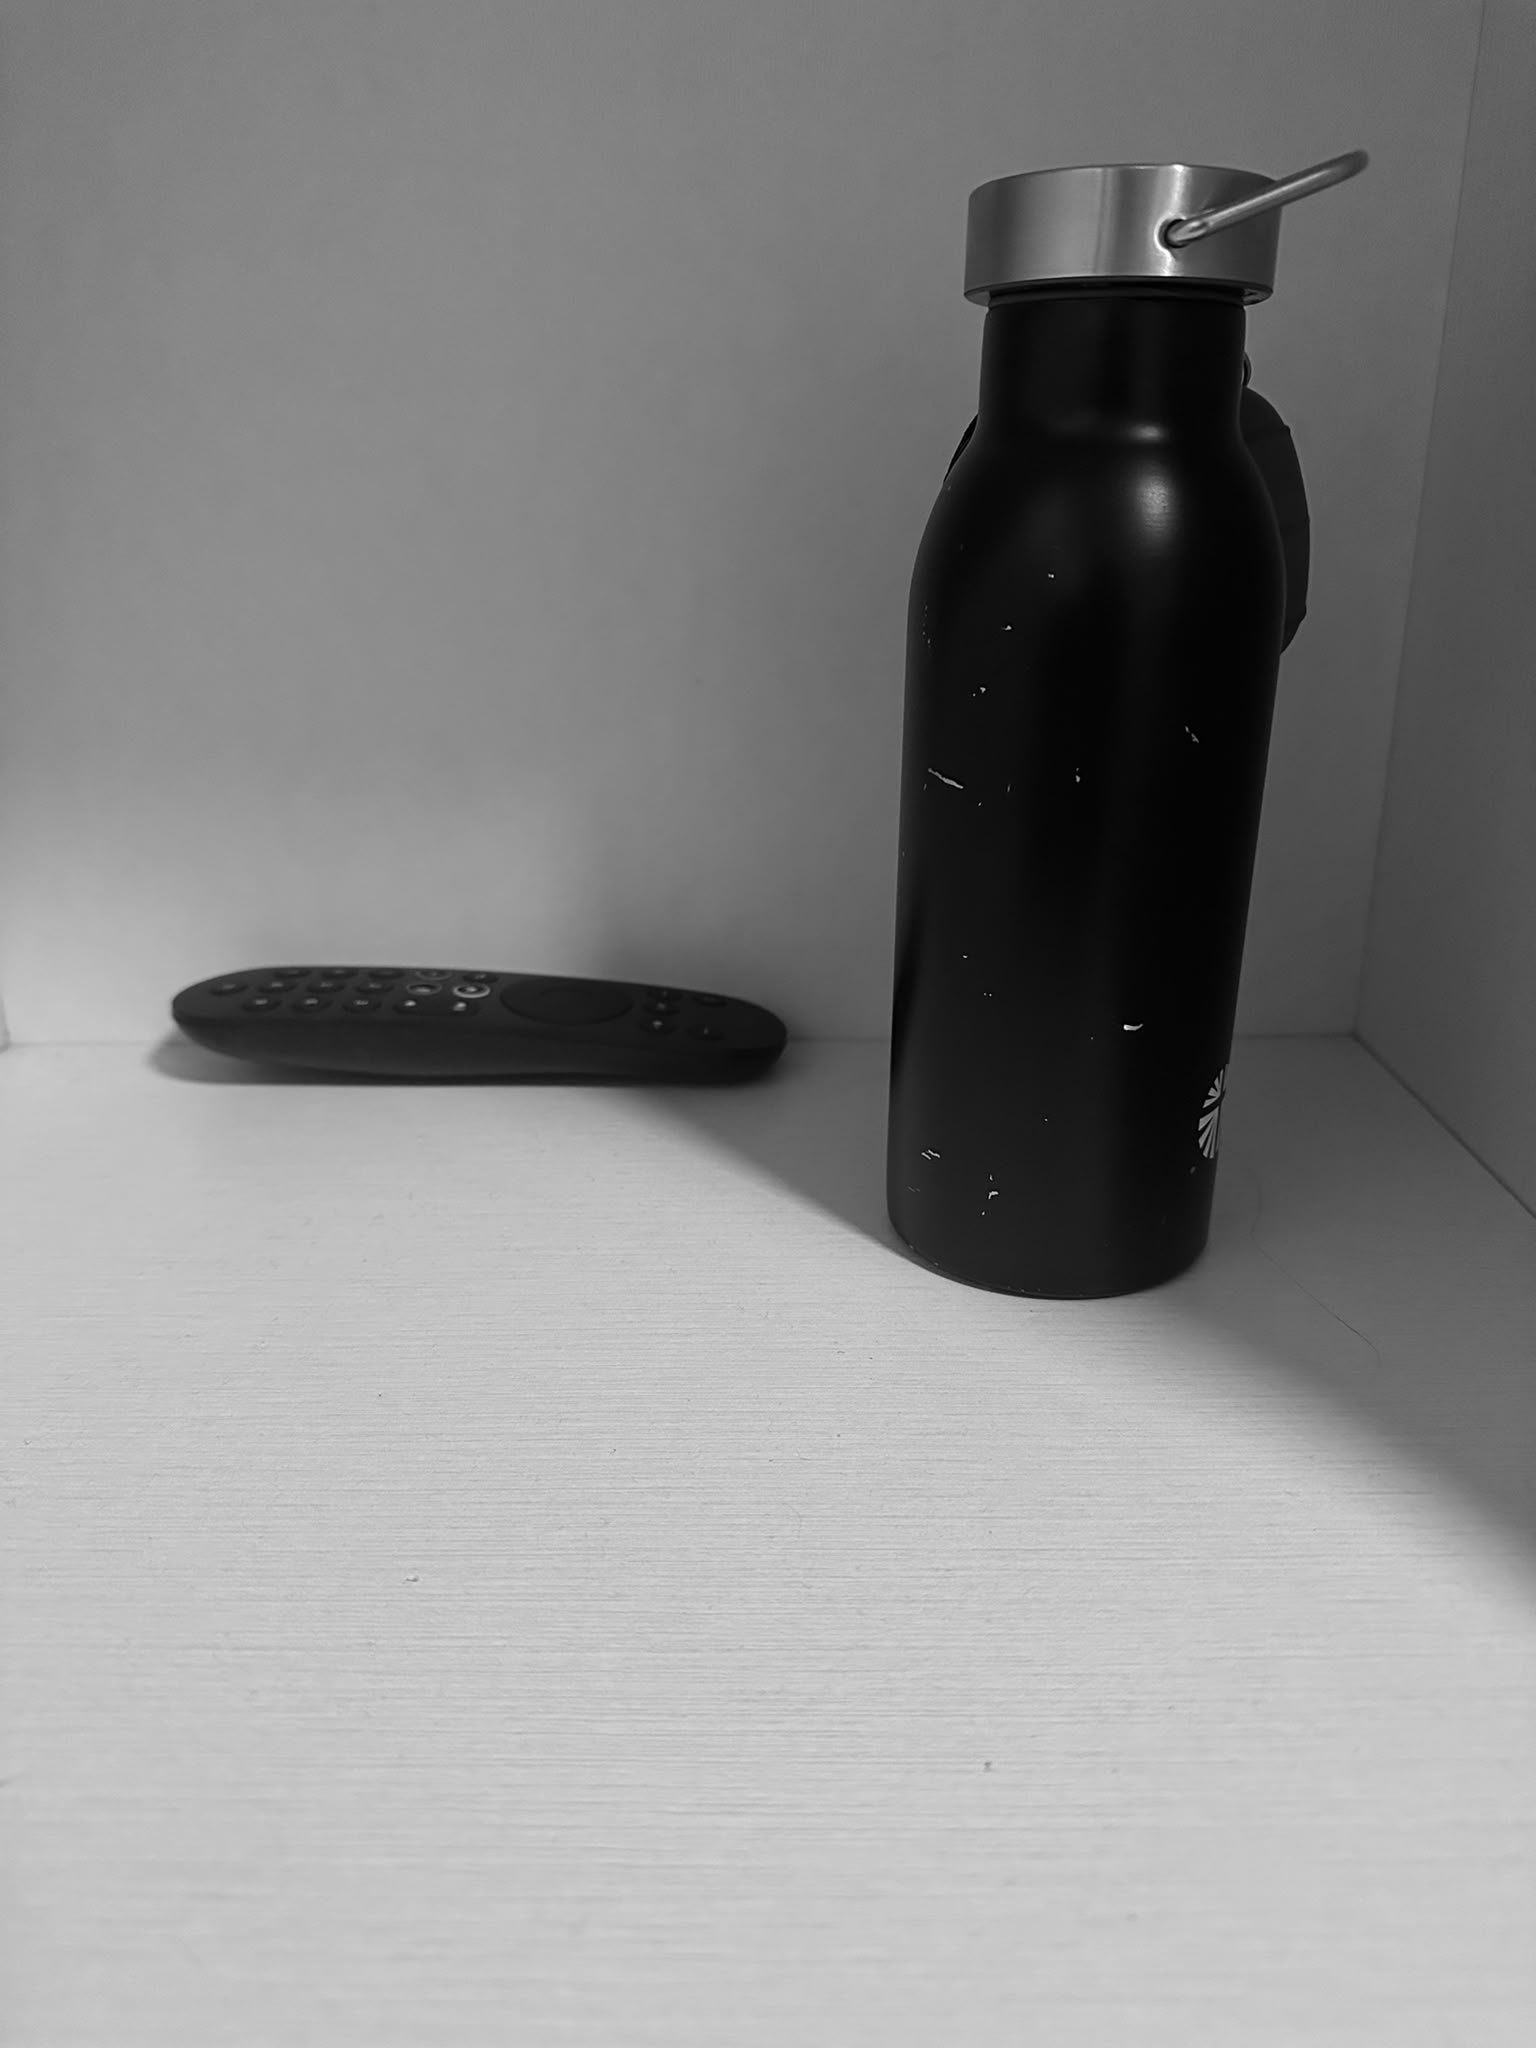
\includegraphics[width=\linewidth]
            {Risorse/Capitolo7/ssim_frame1_grayscale.jpeg}
        \caption{Primo frame in scala di grigi.}
    \end{subfigure}
    \hfill
    \begin{subfigure}[t]{0.39\textwidth}
        \centering
        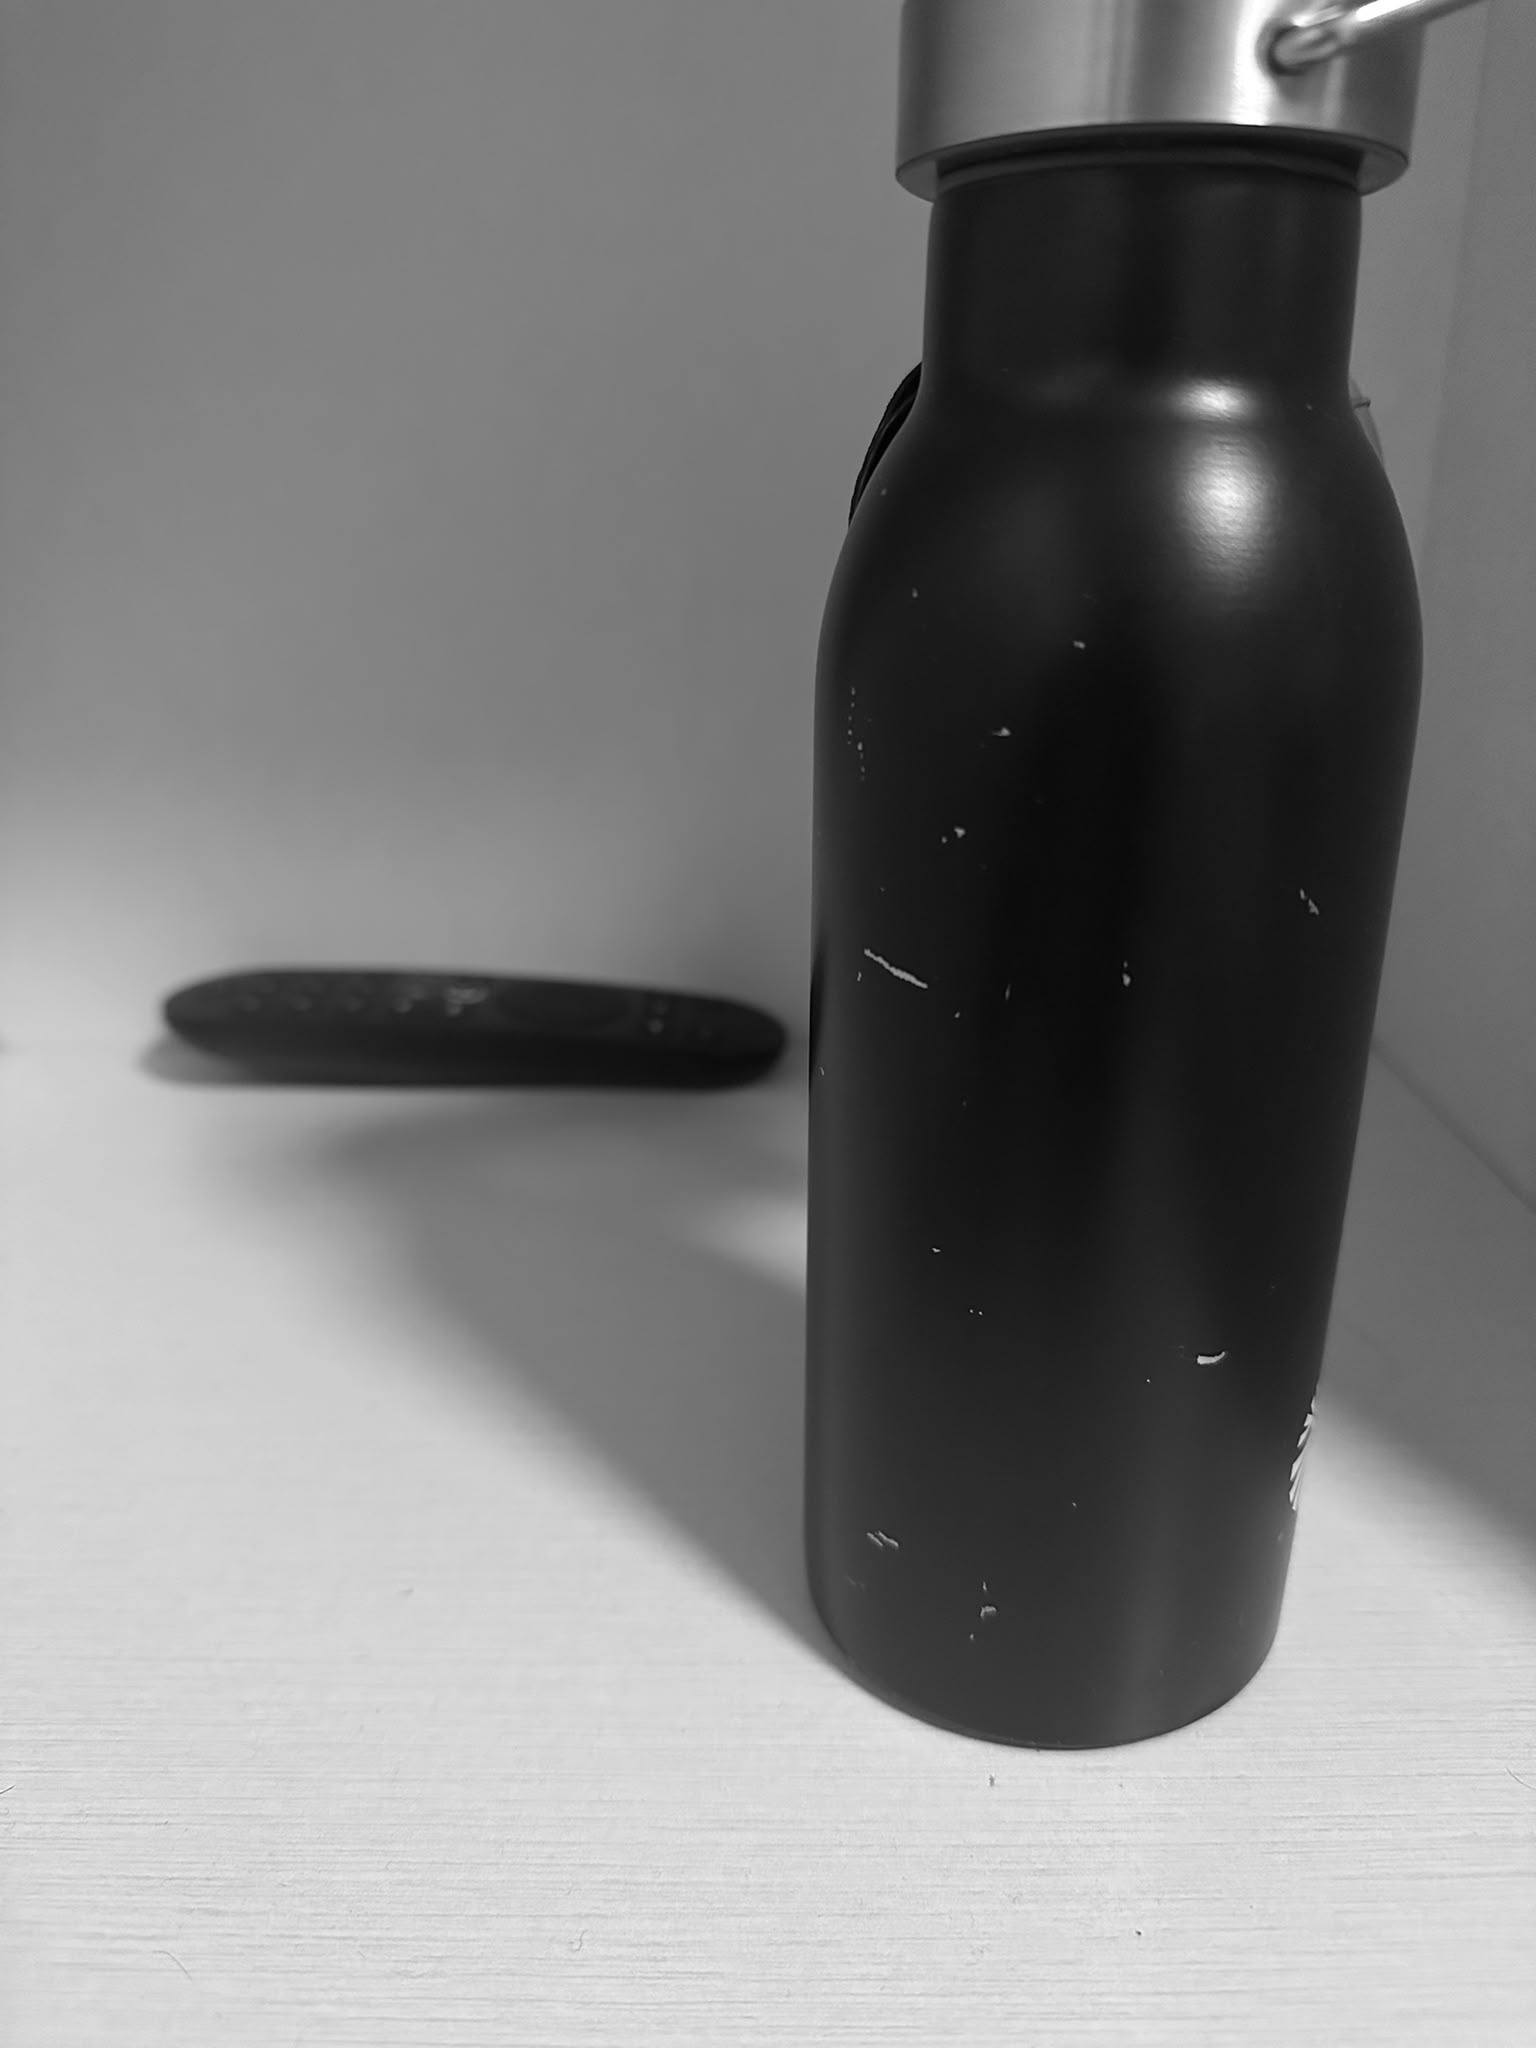
\includegraphics[width=\linewidth]
            {Risorse/Capitolo7/ssim_frame2_grayscale.jpeg}
        \caption{Secondo frame con la bottiglia più vicina.}
    \end{subfigure}

    \vspace{0.8em}

    \begin{subfigure}[t]{0.39\textwidth}
        \centering
        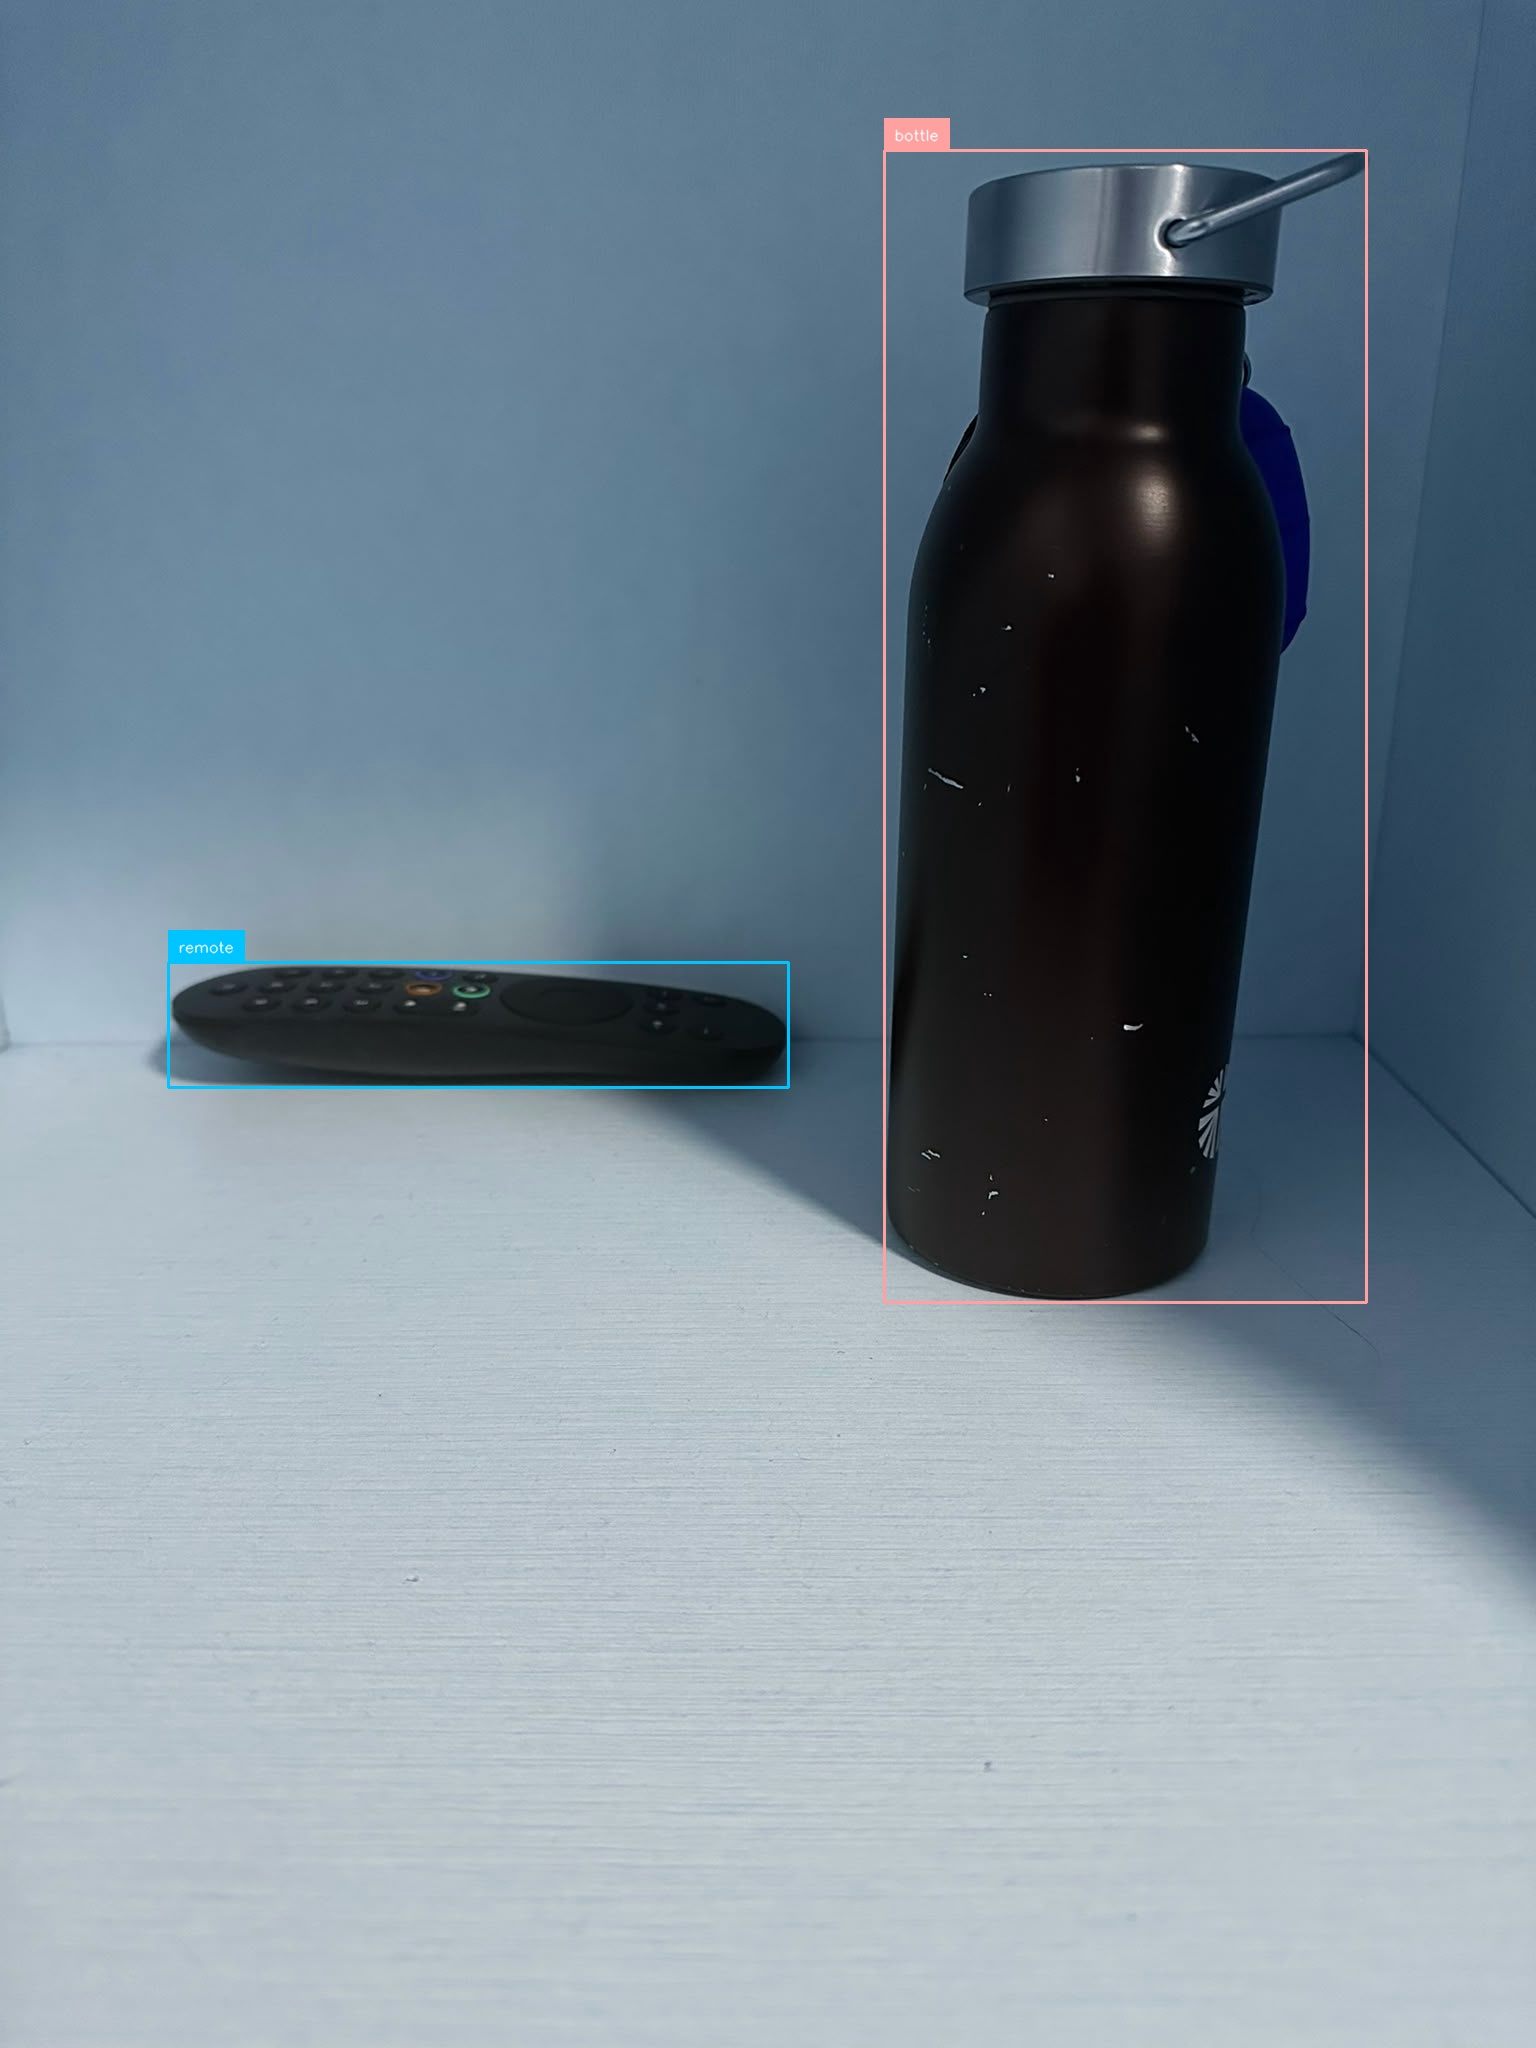
\includegraphics[width=\linewidth]
            {Risorse/Capitolo7/ssim_frame1_rfdetr.jpeg}
        \caption{Detection RF-DETR sul primo frame.}
    \end{subfigure}
    \hfill
    \begin{subfigure}[t]{0.39\textwidth}
        \centering
        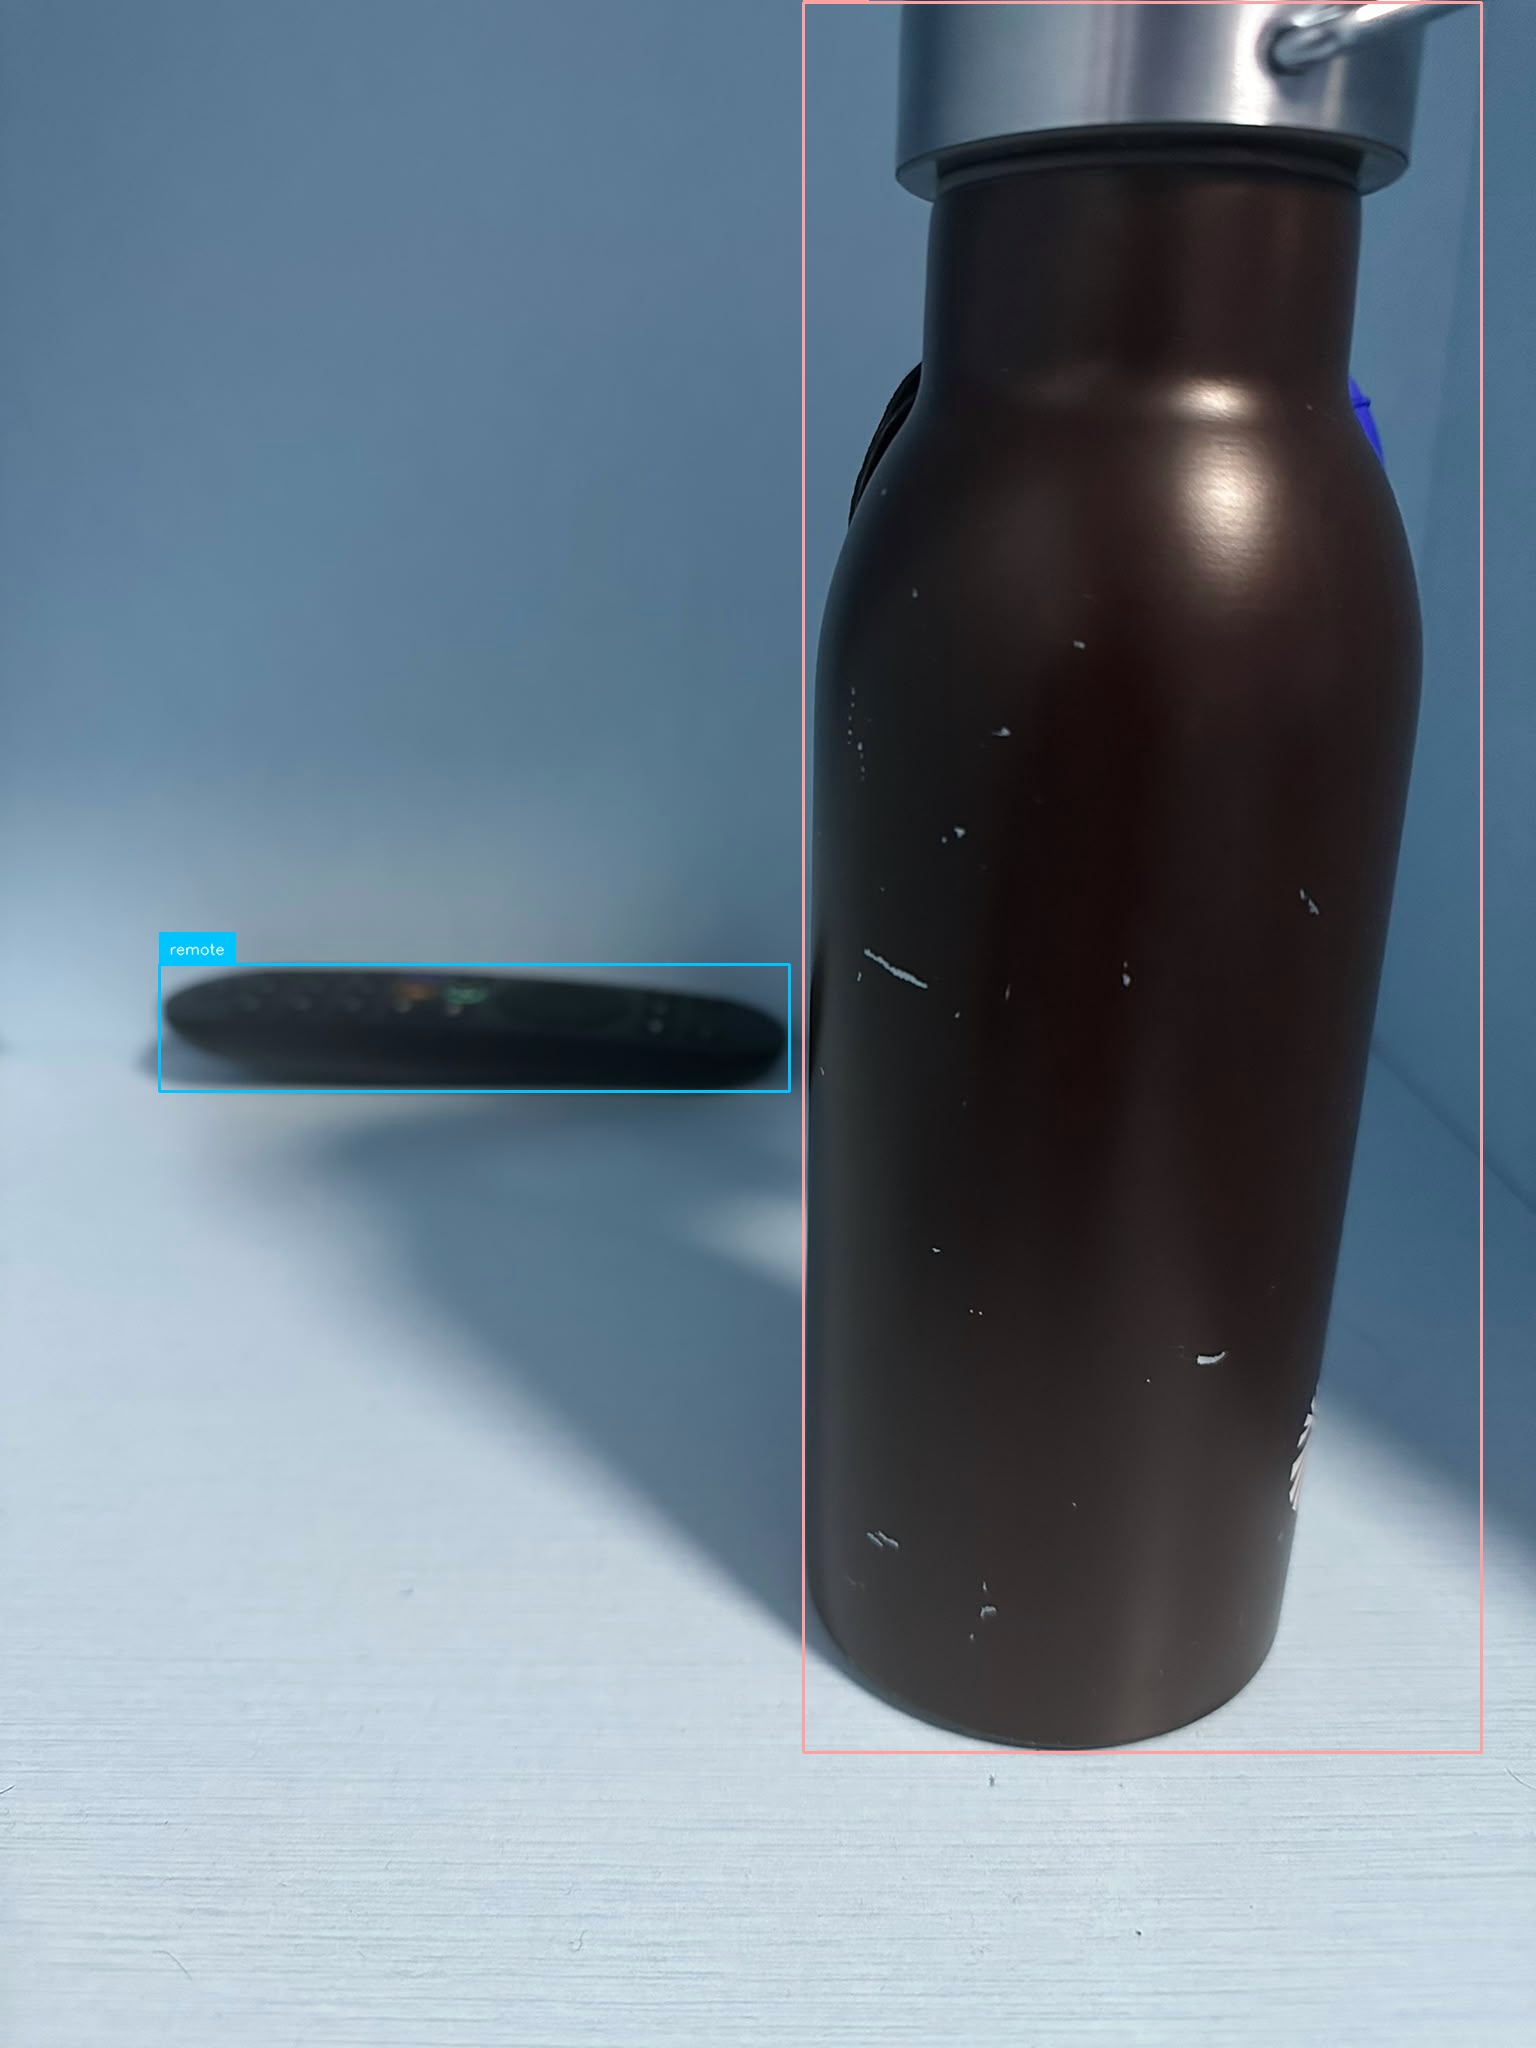
\includegraphics[width=\linewidth]
            {Risorse/Capitolo7/ssim_frame2_rfdetr.jpeg}
        \caption{Detection RF-DETR sul secondo frame.}
    \end{subfigure}
    \caption{Confronto diagnostico tra il controllo strutturale e quello
    semantico. Nonostante il diverso ingombro della bottiglia
    nell'inquadratura, RF-DETR rileva in entrambi i frame una
    \texttt{bottle} e un \texttt{remote}.}
    \label{fig:ssim-dondolio}
\end{figure}

Il confronto tra i due ingressi in scala di grigi ha prodotto uno score SSIM
pari a \(0{,}7924\), con un tempo di \(293{,}7\,\mathrm{ms}\). Poiché la soglia
predefinita del progetto è \(0{,}58\) e il cambiamento viene segnalato soltanto
per valori inferiori alla soglia, questa specifica coppia sarebbe stata
scartata già al primo livello. Nell'esecuzione diagnostica RF-DETR è stato
quindi applicato forzatamente a entrambe le fotografie, ottenendo in entrambi
i casi:

\begin{equation}
    C_1 = C_2 =
    \{\texttt{bottle}: 1,\ \texttt{remote}: 1\}.
    \label{eq:counter-test-ssim-rfdetr}
\end{equation}

Le due inferenze sequenziali di RF-DETR hanno richiesto complessivamente
\(6050{,}6\,\mathrm{ms}\), ossia circa \(3025{,}3\,\mathrm{ms}\) per immagine
in quella singola esecuzione. I tempi devono essere interpretati come misura
diagnostica e non come benchmark generale: le immagini in ingresso erano ad
alta risoluzione, la prova non comprendeva ripetizioni né una fase esplicita
di riscaldamento, e la misurazione del detector escludeva il caricamento
iniziale del modello. Il confronto evidenzia comunque la ragione
architetturale del filtro: evitare l'esecuzione di RF-DETR su ogni frame
ricevuto.

In prove separate, svolte durante il dondolio della fotocamera, sono stati
osservati score SSIM compresi indicativamente tra \(0{,}51\) e \(0{,}65\).
Soltanto i valori inferiori alla soglia attivavano il secondo livello; quando
il \texttt{Counter} delle classi rimaneva invariato, il candidato veniva
soppresso. Introducendo o rimuovendo un oggetto, invece, il conteggio cambiava
e la pipeline proseguiva correttamente.

Il filtro non equivale però a una comprensione completa della scena. Due
inquadrature con le stesse classi e lo stesso numero di istanze possono avere
disposizioni differenti; inoltre un errore del detector può produrre una
variazione artificiale del conteggio. Il meccanismo è quindi una politica di
riduzione dei falsi positivi, non una prova assoluta di equivalenza semantica.

\subsection{Deduplicazione delle caption}
\label{subsec:problemi-deduplicazione}

Anche dopo il filtro sugli oggetti, piccole instabilità delle detection o
formulazioni diverse del VLM potevano produrre frasi quasi equivalenti, ad
esempio ``Un uomo con un telefono'' e ``Un uomo tiene un telefono''. Inviare
entrambe le frasi al TTS comportava un costo aggiuntivo e poteva interrompere
o sovrapporre la riproduzione precedente.

Prima della sintesi, ogni chunk viene quindi confrontato con l'ultimo testo
accettato mediante \texttt{SequenceMatcher}. Indicando con \(S(c_i,c_{i-1})\)
il rapporto di similarità tra il nuovo chunk e il precedente, il TTS viene
saltato quando:

\begin{equation}
    S(c_i,c_{i-1}) > 0{,}85.
    \label{eq:caption-dedup}
\end{equation}

La soglia è configurabile e consente di bilanciare due errori opposti: un
valore troppo basso rischia di sopprimere informazioni nuove espresse con
parole simili; un valore troppo alto lascia passare parafrasi ridondanti.
Inoltre il confronto opera sulla forma testuale e non sul significato
linguistico profondo. Indicando con \(n\) e \(m\) le lunghezze delle due
stringhe, una stima conservativa del costo temporale è
\(\mathcal{O}(nm)\); per caption di lunghezza confrontabile, con
\(n \simeq m\), tale espressione diventa \(\mathcal{O}(n^2)\). La
documentazione di Python precisa che il caso peggiore è quadratico, mentre il
comportamento atteso dipende dalla quantità e dalla disposizione degli
elementi comuni e il caso migliore è lineare
\cite{python314difflib}. Nel contesto applicativo il costo rimane contenuto
perché le caption sono brevi e il confronto non richiede un'ulteriore
inferenza; inoltre esso avviene prima del TTS, evitando il costo molto
maggiore della sintesi quando il testo è ridondante.

\subsection{Gestione del frame di riferimento SSIM}
\label{subsec:problemi-keyframe}

Una seconda criticità riguardava la scelta del riferimento temporale. Nella
prima versione, il frame memorizzato da SSIM veniva aggiornato durante
l'analisi, anche quando il rate limiter impediva alla pipeline di produrre una
caption. Durante una panoramica, il riferimento finiva così per inseguire il
movimento della fotocamera. Quando l'utente si fermava sulla nuova stanza, gli
ultimi due frame risultavano nuovamente simili e il cambiamento poteva non
essere più rilevato. In altre parole, il sistema consumava l'evento mentre il
gate temporale era chiuso.

Per evitare questo comportamento sono state separate due operazioni:

\begin{description}
    \item[\texttt{analyze}] calcola il risultato e conserva il frame e il
    conteggio degli oggetti come candidati;
    \item[\texttt{commit}] consolida il candidato come nuovo riferimento SSIM
    e come nuova memoria semantica.
\end{description}

La pipeline invoca \texttt{commit} soltanto dopo che il cambiamento ha
superato il rate limiter e il controllo di freshness precedente al VLM. Se il
frame viene bloccato da uno di questi gate, il riferimento non avanza e la
scena continua a essere considerata non descritta nei frame successivi.

È opportuno precisare un limite dell'implementazione corrente: il commit
avviene quando il frame viene ammesso alla generazione, prima di conoscere
l'esito finale del VLM e del TTS. Il riferimento rappresenta quindi l'ultimo
frame accettato dalla pipeline di captioning, non necessariamente l'ultimo per
cui l'audio è stato ascoltato. Questa scelta risolve il problema osservato con
il rate limiter, ma lascia spazio a un possibile perfezionamento transazionale
in caso di errore downstream.

\section{Affidabilità dell'interpretazione semantica}
\label{sec:problemi-semantica}

\subsection{Allucinazioni e prolissità del VLM}
\label{subsec:problemi-vlm}

Nelle prime prove il modello
\texttt{meta-llama/llama-3.2-11b-vision-instruct} produceva descrizioni più
lunghe del necessario e introduceva dettagli non sufficientemente supportati
dall'immagine. Tra gli errori osservati figuravano la specificazione
``occhiali da sole'' in presenza di occhiali non chiaramente identificabili,
l'interpretazione di un accessorio come collare e l'attribuzione arbitraria
del tipo di stanza. In un sistema assistivo l'allucinazione è particolarmente
critica: un dettaglio omesso riduce l'informazione disponibile, mentre un
dettaglio inventato può fornire una rappresentazione errata dell'ambiente.

La soluzione ha combinato selezione del modello e controllo della generazione.
Uno script di benchmark ha inviato la stessa immagine e lo stesso prompt a
Gemini 2.5 Flash, GPT-4o-mini, Qwen 2.5 VL, Llama 3.2 Vision e a un'ulteriore
variante Flash. Sul campione utilizzato, Gemini 2.5 Flash ha offerto il
compromesso migliore tra precisione qualitativa e latenza, con un tempo
osservato vicino a \(1{,}9\,\mathrm{s}\). Il valore non costituisce un
benchmark generale del modello: dipende dall'immagine, dal provider, dal
carico di rete e dal momento della richiesta.

Il prompt è stato riscritto includendo vincoli espliciti:

\begin{itemize}
    \item descrivere una sola frase, breve e in italiano;
    \item menzionare soltanto elementi riconosciuti con sufficiente certezza;
    \item usare una categoria generica quando il dettaglio non è distinguibile;
    \item non attribuire un nome all'ambiente se la stanza non è chiaramente
    riconoscibile;
    \item evitare elenchi, intestazioni e formattazione Markdown.
\end{itemize}

Contestualmente, il limite di output della modalità AUTO è stato ridotto da
120 a 80 token e la temperatura da \(0{,}2\) a \(0{,}1\). Queste scelte
riducono la variabilità e la tendenza alla prolissità, ma non possono offrire
una garanzia formale di veridicità. La mitigazione deve pertanto essere
valutata nel Capitolo~\ref{cap:valutazione} mediante un insieme di immagini
più ampio e criteri riproducibili.

\subsection{Vocabolario chiuso di RF-DETR}
\label{subsec:problemi-vocabolario-rfdetr}

Il checkpoint pre-addestrato utilizzato inizialmente opera sulle categorie
COCO. Il task di object detection del dataset comprende 80 categorie di
oggetti \cite{lin2014microsoft_coco}; di conseguenza, un detector
\emph{closed-set} non può assegnare direttamente una classe domestica assente
dal proprio spazio delle etichette. Durante le prove, una stampante è stata
classificata come \texttt{microwave}, cioè come una categoria visivamente
plausibile ma semanticamente errata.

Il problema si propaga oltre la singola bounding box. Le etichette RF-DETR
alimentano il filtro semantico della modalità AUTO: una classe errata può
quindi causare sia descrizioni imprecise sia decisioni sbagliate sulla
presenza di un cambiamento. RF-DETR è progettato anche per l'adattamento a
dataset specifici \cite{robinson2025rfdetr}; la strategia scelta consiste
pertanto nel fine-tuning su categorie quotidiane rilevanti per il dominio
assistivo.

\begin{figure}[H]
    \centering
    % Immagine da acquisire dal detector: una stampante con bounding box,
    % confidence e label errata "microwave". Ritagliare lo sfondo se contiene
    % informazioni personali.
    \IfFileExists{Risorse/Capitolo7/rfdetr_stampante_microonde.jpg}
        {\includegraphics[width=0.70\textwidth]
            {Risorse/Capitolo7/rfdetr_stampante_microonde.jpg}}
        {\fbox{\parbox[c][5cm][c]{0.65\textwidth}{
            \centering
            Inserire il frame di prova nel quale RF-DETR assegna a una
            stampante la classe \texttt{microwave}. Mantenere visibili bounding
            box, etichetta e confidence.
        }}}
    \caption{Esempio di errore causato dal vocabolario chiuso del detector.}
    \label{fig:rfdetr-stampante}
\end{figure}

Nel backend è già presente un adapter capace di caricare un checkpoint
personalizzato e di recuperare i nomi delle classi memorizzati nel modello.
La selezione avviene mediante la variabile
\texttt{RFDETR\_CHECKPOINT}; in sua assenza, il sistema mantiene il fallback
al modello COCO. Sono stati inoltre definiti il processo di costruzione del
dataset, la riconciliazione delle etichette, il fine-tuning e la successiva
reintegrazione.

Questa problematica viene indicata come \emph{in corso}: l'infrastruttura di
caricamento è operativa, ma la qualità del nuovo vocabolario deve essere
dimostrata con un checkpoint addestrato e con metriche calcolate su un test set
separato. Presentare il solo supporto software come soluzione conclusiva
confonderebbe infatti la capacità di caricare un modello con l'effettiva
accuratezza del modello caricato.

\section{Osservabilità della modalità di puntamento}
\label{sec:problemi-pointing}

Quando viene confermato un gesto, il VLM non riceve una sola immagine, ma tre
rappresentazioni complementari dello stesso frame:

\begin{description}
    \item[context] scena completa con corridoio di puntamento sovrapposto;
    \item[focus] area del corridoio evidenziata, sfondo oscurato e ritaglio
    coerente con la geometria;
    \item[clean] immagine originale, utile per verificare il contesto e leggere
    eventuale testo senza sovrapposizioni grafiche.
\end{description}

Inizialmente le trasformazioni avvenivano soltanto in memoria. In presenza di
una descrizione errata non era quindi possibile stabilire se la causa fosse il
raggio geometrico, il ritaglio, la codifica JPEG oppure il ragionamento del
VLM. Salvare tutti i frame non era una soluzione accettabile: avrebbe prodotto
un volume elevato di dati e conservato immagini potenzialmente personali.

È stata introdotta una modalità diagnostica esplicita, disattivata per
impostazione predefinita. Quando
\texttt{POINTING\_DEBUG\_SAVE\_IMAGES} è attivo, il sistema salva le tre
immagini soltanto dopo la conferma del gesto e prima della richiesta al VLM.
I file sono esattamente gli stessi byte JPEG inseriti nel payload multimodale.
Ogni evento utilizza una directory univoca basata su identificativo del frame,
timestamp e suffisso casuale; gli errori di scrittura vengono registrati ma
non interrompono il servizio.

\begin{figure}[H]
    \centering
    % Copiare da una singola cartella artifacts/pointing_debug i tre file
    % prodotti per lo stesso frame. Usare una scena priva di dati personali.
    \begin{subfigure}[t]{0.31\textwidth}
        \centering
        \IfFileExists{Risorse/Capitolo7/pointing_context.jpg}
            {\includegraphics[width=\linewidth]
                {Risorse/Capitolo7/pointing_context.jpg}}
            {\fbox{\parbox[c][3.5cm][c]{0.88\linewidth}{
                \centering
                \texttt{01\_context\_with\_corridor.jpg}
            }}}
        \caption{Contesto e corridoio.}
    \end{subfigure}
    \hfill
    \begin{subfigure}[t]{0.31\textwidth}
        \centering
        \IfFileExists{Risorse/Capitolo7/pointing_focus.jpg}
            {\includegraphics[width=\linewidth]
                {Risorse/Capitolo7/pointing_focus.jpg}}
            {\fbox{\parbox[c][3.5cm][c]{0.88\linewidth}{
                \centering
                \texttt{02\_focus\_darkened\_and\_cropped.jpg}
            }}}
        \caption{Area di interesse.}
    \end{subfigure}
    \hfill
    \begin{subfigure}[t]{0.31\textwidth}
        \centering
        \IfFileExists{Risorse/Capitolo7/pointing_clean.jpg}
            {\includegraphics[width=\linewidth]
                {Risorse/Capitolo7/pointing_clean.jpg}}
            {\fbox{\parbox[c][3.5cm][c]{0.88\linewidth}{
                \centering
                \texttt{03\_clean\_original.jpg}
            }}}
        \caption{Frame originale.}
    \end{subfigure}
    \caption{Le tre viste inviate al VLM nella modalità POINTING.}
    \label{fig:pointing-tre-viste}
\end{figure}

L'export diagnostico risolve contemporaneamente un problema di sviluppo e un
problema metodologico. Permette di riprodurre gli errori e costituisce una
fonte diretta per le figure e per la valutazione sperimentale. La directory
predefinita è esclusa dal controllo di versione e l'acquisizione deve essere
attivata soltanto con scene predisposte e con il consenso delle persone
eventualmente presenti.

\section{Considerazioni conclusive}
\label{sec:problemi-conclusioni}

Le criticità affrontate mostrano che il requisito di tempo reale non coincide
con la sola riduzione della latenza media. VisionCaption ha dovuto controllare
anche l'accumulo dei frame, l'età dell'informazione, la ripetizione delle
caption e la durata dello stato associato a ciascuna connessione. Le soluzioni
più efficaci sono state quindi politiche di selezione e abbandono controllato:
scartare frame intermedi, interrompere elaborazioni scadute e non sintetizzare
testi ridondanti.

Un secondo risultato riguarda la distinzione tra cambiamento visivo e
cambiamento informativo. SSIM rileva efficacemente differenze strutturali, ma
il filtro RF-DETR è necessario per limitare le attivazioni prive di interesse
semantico. A sua volta, il detector è vincolato dal vocabolario con cui è
stato addestrato. La pipeline ibrida riduce quindi una classe di errori senza
eliminare la necessità di valutare dataset e categorie del dominio.

Per la modalità POINTING, l'esportazione diagnostica delle immagini inviate
al VLM consente di collegare ogni risposta alle trasformazioni che l'hanno
prodotta. Questa osservabilità rende verificabile il preprocessing
multimodale senza attribuire a tale intervento la soluzione di una criticità
architetturale diversa.

Rimangono due aspetti da verificare nel Capitolo~\ref{cap:valutazione}: la
generalizzazione delle soglie in condizioni d'uso differenti e l'efficacia
del checkpoint RF-DETR personalizzato su oggetti non presenti nel vocabolario
originario. Questi limiti non invalidano le soluzioni implementate, ma
definiscono con precisione il confine tra il comportamento già verificato e
quello che richiede ulteriori esperimenti.

\chapter{Valutazione sperimentale}
\label{cap:valutazione}

\chapter{Conclusioni e sviluppi futuri}
\label{cap:conclusioni}

\newpage
\chapter{Ringraziamenti}
\begin{itemize}
    \item Prof.ssa Paola Barra
    \item Dott. Antonio Pigna
    \item Giorgia Ibba
    \item Papà
    \item Mamma
    \item Nonni
\end{itemize}
%Come ultimo punto di questa tesi vorrei dedicare questo spazio per ringraziare tutte quelle persone che mi hanno aiutato in un modo o in un altro durante tutto il percorso universitario. \\
%O almeno questo è quello che tutti fanno, ma visto che sono una persona pigra e pragmatica, non scriverò paragrafi di ringraziamenti, ma un elenco di persone che ringrazio. Quindi cominciamo:\\
%\begin{itemize}
%    \item Papà
%    \item Mamma
%    \item Sorè
%    \item Nino
%    \item Pasquale
%    \item Kappa (Flavio)
%    \item Simone
%    \item Claudio
%    \item Inserire nonme di persona random che mi ha iutato nel percorso universitario
%\end{itemize}
%Vi ringazio. 
\newpage
\printbibliography
% Fino a questa riga precedente

\pagestyle{plain}
\end{document}
